%
% Master thesis template for Ghent University (2021)
%
%
%  !!!!!!!!!!!!!!!!!!!!!!!!!!!!!!!!!!!!!!!!!!!!!!!!!!!!!!!!!!!!
%  !!        MAKE SURE TO SET XeLaTex AS LATEX ENGINE        !!
%  !!!!!!!!!!!!!!!!!!!!!!!!!!!!!!!!!!!!!!!!!!!!!!!!!!!!!!!!!!!!
%  !! For overleaf:                                          !!
%  !!     1. click gear icon in top right                    !!
%  !!     2. select `XeLaTex` in "latex engine"              !!
%  !!     3. click "save project settings"                   !!
%  !!                                                        !!
%  !!!!!!!!!!!!!!!!!!!!!!!!!!!!!!!!!!!!!!!!!!!!!!!!!!!!!!!!!!!!
%
%
%  History
%    2014         Doctoral Thesis of Bruno Volckaert
%    2017         Adapted to master thesis by Jerico Moeyersons
%    2018         Cleanup by Merlijn Sebrechts
%    2021         Update by Marleen Denert and Merlijn Sebrechts with feedback from Leen Pollefliet
%    2022         Update by Merlijn Sebrechts
%
%  Latest version
%    https://github.com/galgalesh/masterproef-template
%

% Note: remove `openany` for printed version
\documentclass[11pt,a4paper,openany,english]{book}
\usepackage[a4paper,includeheadfoot,margin=2.50cm]{geometry}




\renewcommand{\baselinestretch}{1.2}  % stretch horizontal space between everything

\usepackage[hyphens]{url} % Break line on hyphens in long urls
\usepackage{graphicx}
\graphicspath{{images/}}
\usepackage{pdfpages}
\usepackage{enumitem}
\usepackage{float}
\usepackage{caption}
\usepackage{subcaption}
\usepackage[toc,page]{appendix}
\usepackage{fontspec}
\usepackage[T1]{fontenc}

% Don't indent table of contents, list of figures, and list of tables
\usepackage{tocloft}
\setlength{\cftsecindent}{0pt}    % Remove indent for \section in Table of Contents
\setlength{\cftsubsecindent}{0pt} % Remove indent for \subsection in Table of Contents
\setlength{\cftfigindent}{0pt}    % remove indentation from figures in List of Figures
\setlength{\cfttabindent}{0pt}    % remove indentation from tables in List of Tables

\usepackage{parskip} % Add space between two paragraphs and don't indent the first line of the paragraph

% To generate fake lorem ipsum text
\usepackage{lipsum}



%
% UGent style guide
%
\setmainfont[
	Path=fonts/,
	BoldFont      =UGentPannoText-SemiBold.ttf,
	ItalicFont    =UGentPannoText-Normal.ttf,
	ItalicFeatures={FakeSlant=0.3},
	BoldItalicFont=UGentPannoText-SemiBold.ttf,
    BoldItalicFeatures={FakeSlant=0.3},
]{UGentPannoText-Normal.ttf}
\urlstyle{same} % Also use the default font for URLs


% If you want left justified text, uncomment the line below.
%\usepackage[document]{ragged2e} % Left justify all text

% Style Chapter titles so they have the chapter number in grey.
\usepackage{color}
\definecolor{chaptergrey}{rgb}{0.5,0.5,0.5}
\usepackage[explicit, pagestyles]{titlesec}
\titleformat{\chapter}[display]{\bfseries}{\color{chaptergrey}\fontfamily{pbk}\fontsize{80pt}{100pt}\selectfont\thechapter}{0pt}{\Huge #1}
\titlespacing*{\chapter}{0pt}{-80pt}{30pt}


% Header showing chapter number and title and footer showing page number
\newpagestyle{fancy}{%
  \sethead{} % left
          {} % center
          {\Large\thechapter~~\chaptertitle} %right
  \setfoot{} % left
          {\thepage} % center
          {} %right
  \setheadrule{0pt}
}
\pagestyle{fancy}

% Header showing chapter title and footer showing page number
\newpagestyle{numberless}{%
  \sethead{} % left
          {} % center
          {\Large\chaptertitle} %right
  \setfoot{} % left
          {\thepage} % center
          {} %right
  \setheadrule{0pt}
}

% We use the package `minted` for modern code highlighting.
\usepackage[newfloat,chapter]{minted}
\SetupFloatingEnvironment{listing}{name=Code Fragment, listname=List of Code Fragments}


\PassOptionsToPackage{hyphens}{url}
\usepackage{hyperref}
\usepackage{url}

\usepackage[numbers]{natbib}       % For bibliography; use numeric citations
\bibliographystyle{IEEEtran}
\usepackage[nottoc]{tocbibind}     % Put Bibliography in ToC

%
% Defines \checkmark to draw a checkmark
%
\usepackage{tikz}
\def\checkmark{\tikz\fill[scale=0.4](0,.35) -- (.25,0) -- (1,.7) -- (.25,.15) -- cycle;}

%
% For tables
%
\usepackage{booktabs}
\usepackage{array}
\usepackage{ragged2e}  % for '\RaggedRight' macro (allows hyphenation)
\newcolumntype{L}[1]{>{\raggedright\let\newline\\\arraybackslash\hspace{0pt}}m{#1}}
\newcolumntype{C}[1]{>{\centering\let\newline\\\arraybackslash\hspace{0pt}}m{#1}}
\newcolumntype{R}[1]{>{\raggedleft\let\newline\\\arraybackslash\hspace{0pt}}m{#1}}

\usepackage{polyglossia}
\setmainlanguage{english}

% Fix error "Package hyperref Warning: The anchor of a bookmark and its parent's must not be the same. Added a new anchor on ..."
\newcommand{\sectionbreak}{\phantomsection}

\usepackage[toc,acronym]{glossaries}  % for list of acronyms
\makeglossaries                       % start internal list of acronyms


%
% Set the title and your name
%
%%%%%%%%%%%%%%%%%%%%%%%%%%%%%%%%%%%%%%%%%%%%%%%%%%%%%%%%%%%%%%%%%%%%%%
%
% Add the specific info for your thesis
%
%%%%%%%%%%%%%%%%%%%%%%%%%%%%%%%%%%%%%%%%%%%%%%%%%%%%%%%%%%%%%%%%%%%%%%

\title{Discovering Digital Art Collections using Link-Traversal-based Query Processing}
\author{Martijn Bogaert}

%%%%%%%%%%%%%%%%%%%%%%%%%%%%%%%%%%%%%%%%%%%%%%%%%%%%%
% Add all the acronyms you use in your thesis here. %
% These will be added to the List of Acronyms       %
%%%%%%%%%%%%%%%%%%%%%%%%%%%%%%%%%%%%%%%%%%%%%%%%%%%%%

\newacronym{LD}{LD}{Linked Data}
\newacronym{LTQP}{LTQP}{Link-Traversal-based Query Processing}
\newacronym{IIIF}{IIIF}{International Image Interoperability Framework}
\newacronym{RDF}{RDF}{Resource Description Framework}
\newacronym{RDFS}{RDFS}{Resource Description Framework Schema}
\newacronym{OWL}{OWL}{Web Ontology Language}
\newacronym{JSON}{JSON}{JavaScript Object Notation}
\newacronym{JSON-LD}{JSON-LD}{JavaScript Object Notation for Linked Data}
\newacronym{HTML}{HTML}{HyperText Markup Language}
\newacronym{URI}{URI}{Uniform Resource Identifier}
\newacronym{HTTP}{HTTP}{Hypertext Transfer Protocol}
\newacronym{HTTPS}{HTTPS}{Hypertext Transfer Protocol Secure}
\newacronym{DNS}{DNS}{Domain Name System}
\newacronym{SPARQL}{SPARQL}{SPARQL Protocol and RDF Query Language}
\newacronym{FOAF}{FOAF}{Friend of a Friend}
\newacronym{CoGhent}{CoGhent}{Collections of Ghent}
\newacronym{N3}{N3}{Notation3}
\newacronym{XML}{XML}{Extensible Markup Language}
\newacronym{HMO}{HMO}{Human-Made Object}
\newacronym{DMG}{DMG}{Design Museum Gent}
\newacronym{HVA}{HVA}{Huis van Alijn}



%
%  END OF HEADER
%  The actual latex document content starts here.
%
\begin{document}
\frontmatter
\pagestyle{empty}

% Download the cover sheet from Plato
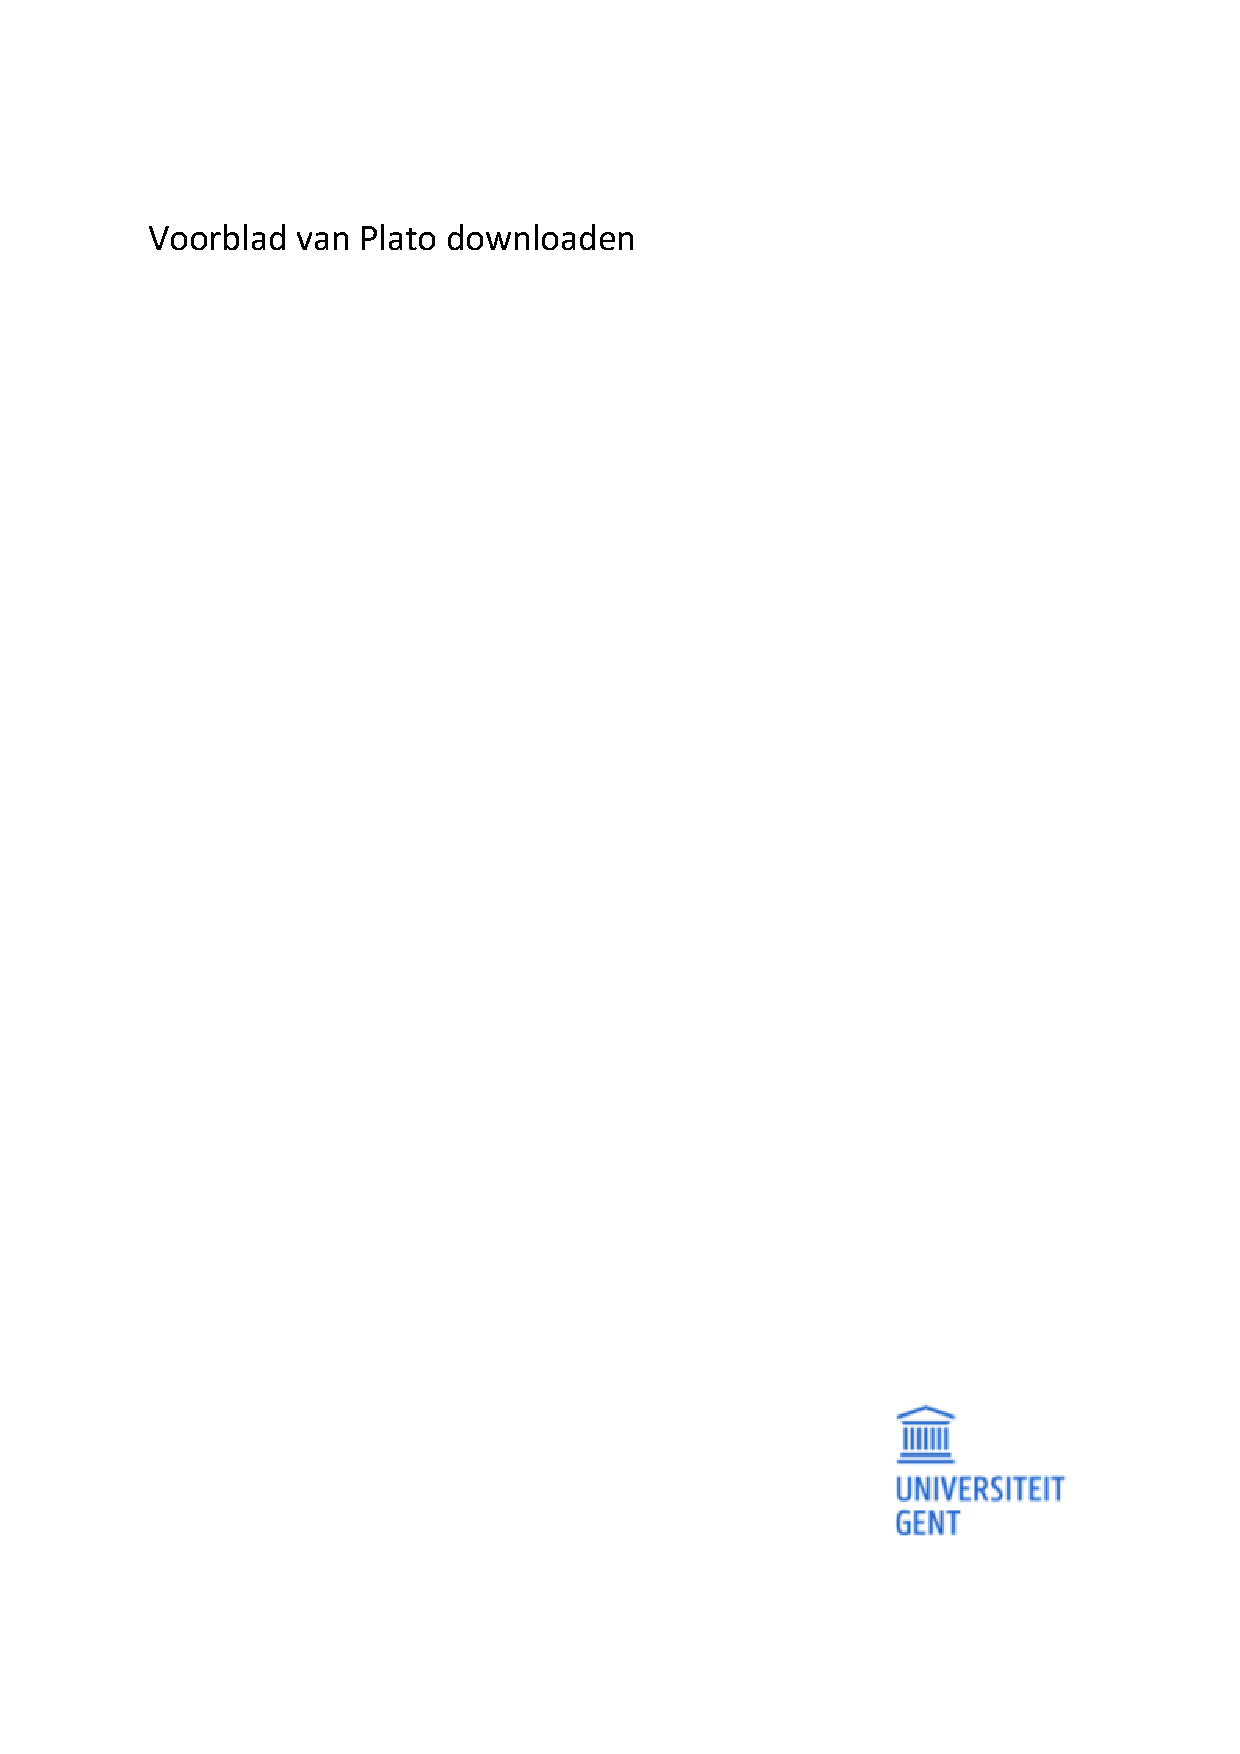
\includepdf{cover-sheet.pdf}

\pagestyle{plainpage}

\chapter*{Acknowledgements}

There are many people I would like to thank for their valuable advice and support over the past months. During those months, I have had the privilege of immersing myself in what has been an entirely new world for me, at the same time collaborating with very talented people. However, the past months have also been challenging. Therefore, a heartfelt thank you to those who have helped me navigate through them, is more than fitting.

First and foremost, I would like to express my sincere gratitude to Bryan-Elliott Tam. Bryan was my counselor throughout the second and third semesters of the academic year, going above and beyond to navigate me through the realm of link traversal. I distinctly recall one of our initial meetings. Bryan had prepared an entire PowerPoint presentation to help me get started with the new approach for my thesis, which we had decided on just the week before. I was able to dive right in. However, what I am most thankful to Bryan for, are his numerous reassuring and encouraging words during the more challenging moments. Especially during the last month, it brought me a great deal of comfort. So, Bryan, from the bottom of my heart: thank you.

Omdat ik met de volgende mensen in het dagelijkse leven steeds in mijn moedertaal communiceer, schakel ik even over naar het Nederlands. Dat doe ik in eerste instantie om Brecht Van de Vyvere te bedanken. Brecht was mijn begeleider tijdens het eerste semester van het academiejaar en heeft me mijn eerste stappen in de wereld van Linked Data helpen zetten. Dat deed hij altijd met veel zorg en de grootste glimlach. Dankjewel, Brecht.

Iemand die ik zeker niet mag en kan vergeten te bedanken, is Olivier Van D'huynslager. Als digitaal hoofd van CoGent heeft Olivier me bijna een volledig jaar lang mee begeleid. Op bijna elke meeting die ik met mijn begeleider hield, was Olivier aanwezig. Hij nam die extra vergaderingen er met de glimlach bij. Bedankt voor al je ideeën en goede raad, Olivier.

Ook Pieter Colpaert wil ik bedanken. Hij was anderhalf jaar geleden degene die me tijdens een wandeling in de Blaarmeersen kennis liet maken met de wereld van Linked Data. Dat deed hij met veel overgave en passie. Ik hoefde dan ook niet lang te twijfelen welk masterproefonderwerp ik zou kiezen. Bedankt, Pieter.

Dan zijn we aangekomen bij mijn familie. Ik ga het mezelf niet te moeilijk maken en meteen met mijn ouders beginnen. Zij zullen namelijk ook gemerkt hebben dat dit laatste jaar voor mij veruit de meest uitdagende van de voorbije zes was. Gelukkig heb ik de beste ouders die iemand zich kan wensen, en stonden zij trouw op de eerste rij om me er met aanmoedigende woorden en veel liefde doorheen te loodsen. Mama en papa, ik zal het jullie nog wel luidop zeggen, maar hier staat het alvast zwart op wit: dankjewel.

Wie ook zeker niet mag ontbreken op deze pagina, zijn mijn grootouders. Niet alleen tijdens het schrijven van mijn masterproef, maar jarenlang, tijdens elke examenperiode, mocht ik bij hen - gewoon het hoekje om - in alle rust komen werken. Elke dag opnieuw werd ik beladen met lekker eten, tussendoortjes, aanmoedigingen en vooral veel liefde. Ik heb veel onvergetelijke momenten meegemaakt tijdens mijn studententijd, maar ik lieg niet als ik zeg dat ik de dagen bij hen nog het meest zal missen. Lieve moemoe en grootva, ik ben jullie eeuwig dankbaar.

En dan is er nog iemand die ongetwijfeld niet kan wachten haar naam te horen. Mijn allerliefste Eva, dankjewel voor al die weken, maanden en jaren onophoudelijke steun. Ik weet niet hoe je het doet, maar zelfs op de moeilijkste momenten slaag je er telkens weer in mij op te rapen en met nieuwe moed vooruit te doen kijken. Ik kan niet wachten om met jou de volgende fase van mijn - ons - leven te beginnen. Ik zie je graag.

Ten slotte wil ik ook alle mensen die ik nog niet vermeld heb maar die me toch al die tijd gesteund hebben, heel oprecht bedanken. Ik denk daarbij aan familie, vrienden, medestudenten ... Die steun hoeft zelfs niet altijd uitgesproken te zijn. Een schouderklopje of een aanmoedigende glimlach kan al een wereld van verschil maken. Het zijn de kleine gebaren die het 'm doen. Dankjewel allemaal!
\chapter*{Toelichting in verband met het masterproefwerk}

Deze masterproef vormt een onderdeel van een examen. Eventuele opmerkingen die door de beoordelingscommissie tijdens de mondelinge uiteenzetting van de masterproef werden geformuleerd, werden niet verwerkt in deze tekst.

% This master's dissertation is part of an exam. Any comments formulated by the assessment committee during the oral presentation of the master's dissertation are not included in this text.

\subsection*{Melding van vertrouwelijkheid (enkel indien van toepassing)}

Bekijk hiervoor de informatie op \href{https://www.ugent.be/ea/nl/faculteit/studentenadministratie/masterproef/} {de facultaire website} - \textbf{Nota in verband met de vorm van de masterproef (alle opleidingen)}
\chapter*{Abstract}
\chaptermark{Abstract}
\addcontentsline{toc}{chapter}{Abstract}

\section*{English}

This master's thesis explores the innovative approach of discovering digital art collections using Link-Traversal-based Querying, focusing on the Collections of Ghent (CoGhent) data. CoGhent, a former partnership that digitized collections from cultural institutions, published the data as Linked Data in RDF format. By employing link traversal, this data can be explored in new ways, offering fresh insights into art collections.

The Comunica platform is central to this process, allowing for link traversal of RDF datasets and enabling the extraction of valuable data. In the CoGhent data, for instance, each entity referred to as a \textit{Human-Made Object}, such as an art piece, links to a IIIF Manifest. This manifest is a JSON-LD document that specifies artwork data and may provide instructions for digital display. Particularly, it holds a link to a picture of the piece, offering a visual representation of the artwork.

However, some resource links in the CoGhent data, notably Getty Vocabularies links, do not return an RDF compliant document, presenting a challenge for the Comunica link traversal engine. Workarounds are needed to reach the RDF compliant counterparts of these non-RDF compliant documents.

To make the discovery of CoGent collections accessible and assist art enthusiasts or professionals without a technical background in constructing SPARQL queries for a link traversal engine, two web application ideas are proposed. The first allows users to select predetermined properties of artworks, accompanied by a question indicating the purpose of the property. Each property corresponds to a sequence of predicates, which the application can ultimately use to generate a query. The second idea enables users to start from a resource of their choice, build a tree of predicates and objects, and eventually select objects of interest for query construction.

Ultimately, the discovered data can be incorporated in a IIIF Manifest, allowing display using a IIIF Viewer. This approach enhances the accessibility of art collections and provides a novel way to explore the rich cultural heritage in the CoGhent data.

\newpage
\newpagestyle{plainpage}{
  \sethead{}{}{}
  \setfoot{}{\thepage}{}
  \setheadrule{0pt}
}
\pagestyle{plainpage}

\section*{Nederlands}

Deze masterproef onderzoekt hoe digitale kunstcollecties met behulp van Link-Traversal-based Querying verkend kunnen worden. De focus ligt daarbij op de data die gepubliceerd werd door de Collectie van de Gentenaar (CoGent). Dit gewezen samenwerkingsverband digitaliseerde collecties van culturele instellingen en publiceerde de gegevens als Linked Data in RDF-formaat. Door link traversal te gebruiken, kunnen deze gegevens op nieuwe manieren worden verkend, wat leidt tot nieuwe inzichten in kunstcollecties.

Het Comunica-platform speelt een centrale rol in dit proces. Het maakt link traversal van RDF-datasets mogelijk, waardoor waardevolle gegevens kunnen worden verkregen. In de CoGent-data, bijvoorbeeld, verwijst elke entiteit die wordt aangeduid als een \textit{Mensgemaakt Object}, zoals een kunstwerk, naar een IIIF Manifest. Dit manifest is een JSON-LD-document dat kunstwerkgegevens specificeert en mogelijk instructies geeft voor digitale weergave. In het bijzonder bevat het een link naar een afbeelding van het stuk.

Echter, sommige resource-links in de CoGent-data, met name Getty Vocabularies-links, geven geen RDF-conform document terug. Hier kan Comunica niet mee aan de slag. Er zijn dus oplossingen nodig om de RDF-conforme tegenhangers te bereiken.

Om de ontdekking van CoGent-collecties toegankelijk te maken en kunstliefhebbers of professionals zonder technische achtergrond te helpen bij het opstellen van SPARQL-queries voor een link traversal engine, worden twee ideeën voor webapplicaties voorgesteld. Het eerste stelt gebruikers in staat om vooraf bepaalde eigenschappen van kunstwerken te selecteren, vergezeld van een vraag die het doel van de eigenschap aangeeft. Elke eigenschap komt overeen met een aaneenschakeling van predicaten, waarmee de applicatie uiteindelijk een query kan genereren. Het tweede idee stelt gebruikers in staat om vanuit een resource naar keuze, een boom van predicates en objecten op te bouwen, en finaal objecten van belang te selecteren voor queryconstructie.

Uiteindelijk kunnen de ontdekte gegevens worden toegewezen aan een IIIF Manifest, waarna een IIIF Viewer ze kan visualiseren. Deze benadering vergroot de toegankelijkheid van kunstcollecties en biedt een nieuwe manier om het rijke culturele erfgoed in de CoGent-data te verkennen.
% Write the extended abstract as a separate project using the IEEE conference proceedings template, and include the resulting PDF here in the document. You can find the template on Overleaf: https://www.overleaf.com/latex/templates/ieee-conference-template/grfzhhncsfqn. 

%Voeg dit toe als .pdf
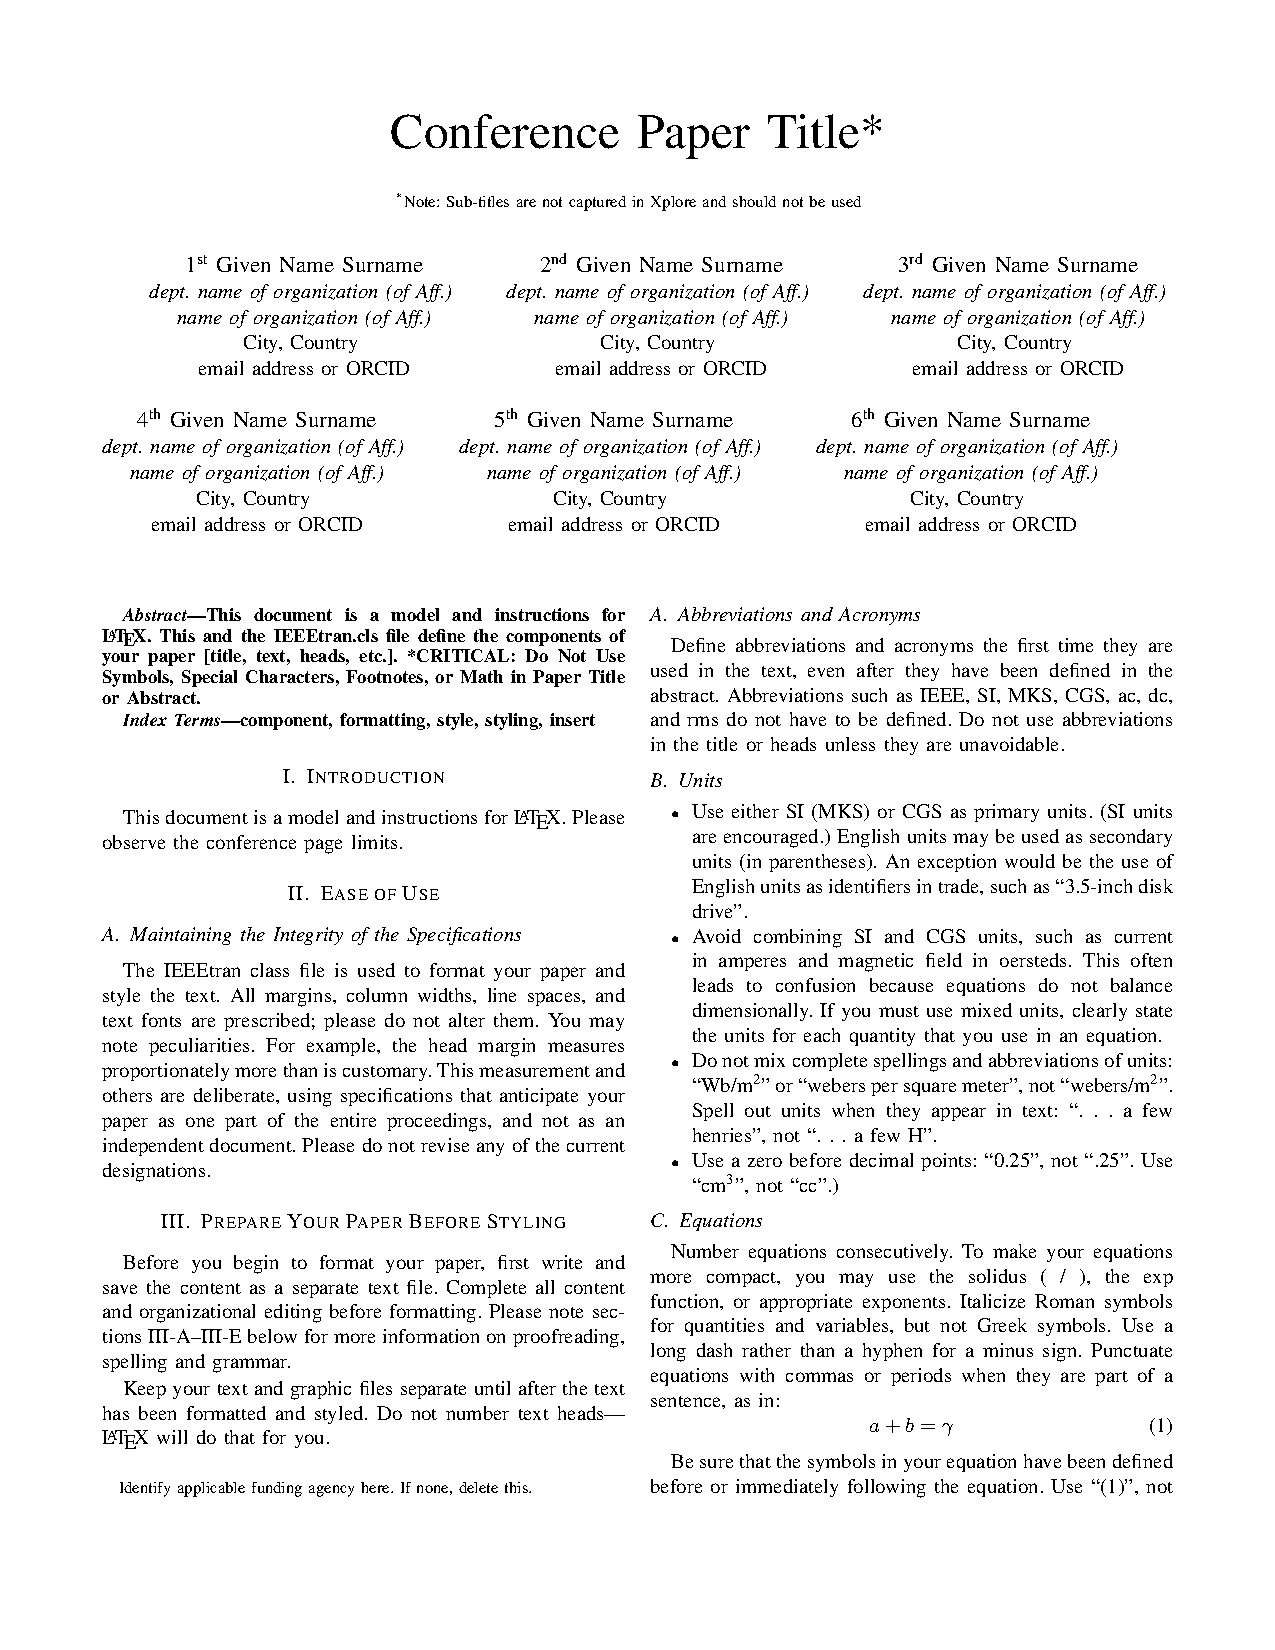
\includepdf[pages={-}]{abstract.pdf}  % Extended Abstract

\tableofcontents\newpage
\listoffigures\newpage
\listoftables\newpage
%%%%%%%%%%%%%%%%%%%%%%%%%%%%%%%%%%%%%%%%%%%%%%%%%%%%%%%%%%%%%%%
%                                                             %
% Note: To add or remove acronyms, modify `personal_data.tex` %
%                                                             %
%%%%%%%%%%%%%%%%%%%%%%%%%%%%%%%%%%%%%%%%%%%%%%%%%%%%%%%%%%%%%%%


% Print the glossary
\printglossary[type=\acronymtype, title={List of Acronyms}]

\glsaddallunused[\acronymtype]                              % make sure all unused acronyms are in list

\setlist[description]{style=standard} % reset list settings back to default

\listoflistings\newpage

%
% Include the main chapters of the thesis below
% Note: it's best to avoid spaces in filenames as Latex might complain about them.
%
\mainmatter
\pagestyle{fancy} % Use header
\chapter*{Introduction}
\chaptermark{Introduction}
\addcontentsline{toc}{chapter}{Introduction}

Digital art collections have long stood as a testament to human creativity and cultural evolution. With the advent of technology, many of these collections have undergone digitization, making them more accessible to a global audience. This digitization not only preserves the integrity of the artworks but also offers an opportunity for deeper exploration and understanding. However, with this digital transformation comes a set of challenges, especially for those without a technical background. Professionals in the cultural domain and general art enthusiasts, while passionate about art, may not possess the technical expertise to navigate and query these digitized datasets. This limitation can hinder their ability to make new discoveries and truly immerse themselves in the digital art world.

Discovering art collections can be interpreted in myriad ways. At its core, discovery is about unearthing new insights, understanding the nuances of each artwork, and drawing connections that might not be immediately apparent. This research primarily focuses on retrieving the inherent properties of cultural objects, delving into the intricate details that make each piece unique. However, the true potential of discovery lies in going beyond the confines of a single dataset. Link traversal offers this opportunity, allowing for a broader exploration that extends beyond the immediate dataset, unveiling new layers of knowledge and understanding.

By employing link traversal, one can uncover hidden relationships, gain a deeper understanding of cultural objects, and even compare different artworks in novel and enlightening ways. This approach is particularly beneficial when exploring the Collections of Ghent (CoGhent), a collaborative initiative between various cultural institutions. Published in a Linked Data format, the CoGhent collections are primed for link traversal, enabling a richer and more comprehensive exploration.

This research situates itself at the intersection of art and technology, aiming to bridge the gap between the two. It seeks to empower both professionals and art enthusiasts to navigate the digital art landscape, harnessing the power of link traversal to make new discoveries and draw meaningful connections. Through a systematic exploration of the Collections of Ghent and the development of tools tailored for query formulation, this research offers a roadmap for discovering digital art collections in their entirety.

Chapter~\ref{chap:rel_work} elucidates the foundational concepts of Linked Data and their real-world applications. It delves into the core principles, data modeling, and various RDF syntaxes, setting the stage for a deeper exploration of link traversal in the subsequent chapters. 

Chapter~\ref{chap:coghent_link_traversal} focuses on the CoGhent collections, highlighting the potential of link traversal for discovering properties of Human-Made Objects. It provides an overview of the available data sources and the development of a link traversal engine optimized for the objectives of this research.

In Chapter~\ref{chap:tools_query_building}, the emphasis shifts to the development of user-centric tools for query formulation. Two conceptual web applications are introduced, designed to alleviate the technical complexities of query formulation for users. The chapter also discusses the fundamental functionality shared by both web applications, ensuring a cohesive exploration throughout.

Lastly, Chapter~\ref{chap:handling_query_results} addresses the challenges of visualizing and preserving query results. It offers an overview of potential solutions, outlining their advantages and drawbacks, ensuring that the treasures within the CoGhent collections are accessible and meaningful to all.
\chapter{Related work}
\label{chap:rel_work}

\section{Linked Data}

This section presents a comprehensive exploration of Linked Data, encompassing its fundamental principles, data modeling, syntax, query interfaces, and the associated challenges and advantages. In Section~\ref{subsec:introduction_principles}, the concept of Linked Data and its principles are introduced, highlighting the significance of unique URIs, dereferencing, and data interlinking. Section~\ref{subsec:rdf} focuses on the Resource Description Framework (RDF) as the cornerstone for representing relationships and knowledge connections within Linked Data. Section~\ref{subsec:rdf_syntax} provides an overview of RDF syntax, including popular formats such as XML, Turtle, N-Triples, and JSON-LD, which facilitate the flexible expression and exchange of RDF data. Section~\ref{subsec:rdfs_owl} explores the Resource Description Framework Schema (RDFS) and Web Ontology Language (OWL), enabling the extension of Linked Data through ontology definition and enhanced semantic representation. Section~\ref{subsec:sparql} delves into SPARQL, the query language for Linked Data, and discusses various query interfaces that facilitate efficient data access and retrieval. Lastly, Section~\ref{subsec:challenges_advantages} examines the challenges and advantages of Linked Data, addressing aspects such as data quality, scalability, integration, and the benefits of improved interoperability and knowledge graph creation. This comprehensive examination provides a solid foundation for the subsequent discussions on linked traversal-based query processing.

\subsection{Introduction and Principles}
\label{subsec:introduction_principles}

To better understand the origins of the idea behind Linked Data, it is important to examine the origins of the World Wide Web. For example, its first, but still rather primitive, underlying technology was introduced in 1989 at CERN. Tim Berners-Lee was the man responsible for its development. By using HyperText Markup Language (HTML), it enabled scientists, and later the rest of the world, to publish documents that could contain links to other documents. This helped create a mesh of documents and information. However, since these documents in fact contained nothing more than raw data dumps and links between documents represented simply an indication of how to reach the document, these documents and their relationships lacked semantics. Figure~\ref{fig:no_linked_data} illustrates what a web of documents without unambiguous indications of what their contents and the links between them represent, might look like. It is necessary to note here that the used icons are not the contents of their respective documents, but only a representation of their contents. Nevertheless, in themselves, they prove the weakness of such web as much as when the effective content of the documents had been represented. After all, just from the raw content of documents and their mutual links, a person cannot clearly infer exactly what their constellation represents, let alone a computer. From that deficiency, therefore, emerged the idea of Linked Data. \citep{jacksi2019development} \citep{bizer2011linked}

\begin{figure}[htbp]
    \centering
	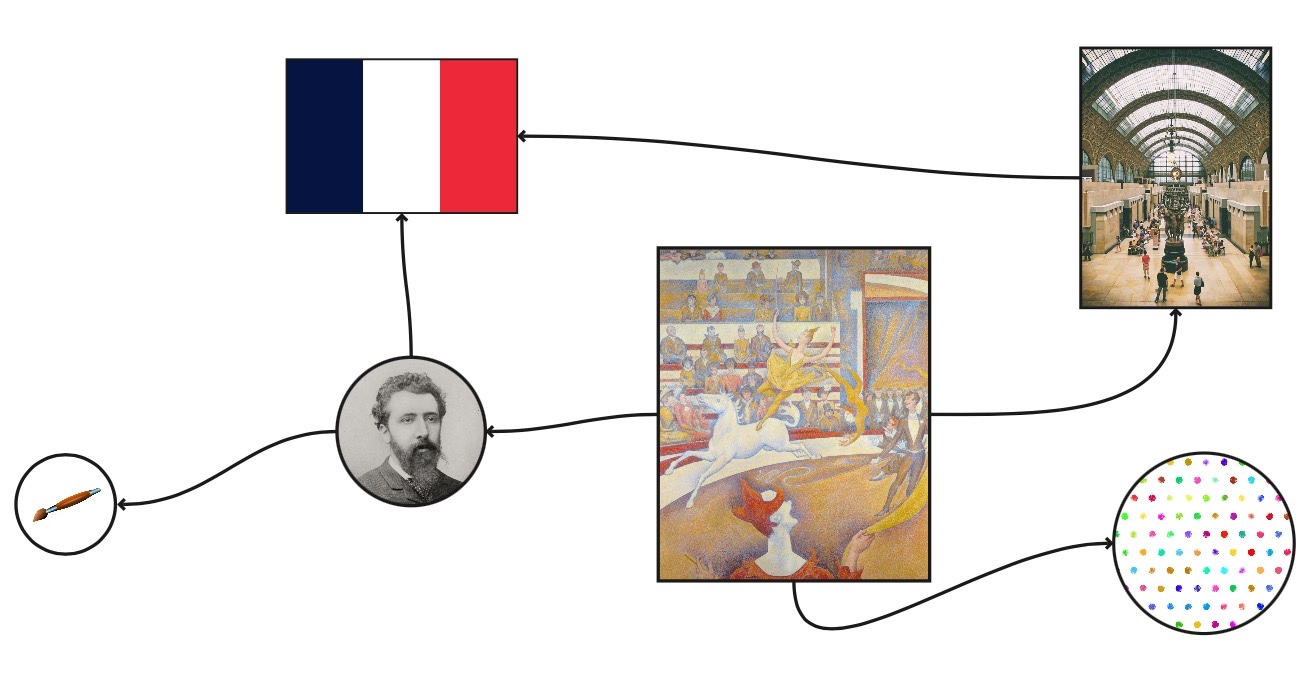
\includegraphics[width=\textwidth]{images/no_linked_data.jpg}
    \captionsetup{justification=centering}
	\caption{Representation of a web of documents without unambiguous indications of what the documents and the links between them represent}
	\label{fig:no_linked_data}
\end{figure}

Simply put, data coming from different sources can be labeled as Linked Data as soon as they are linked by typed links. In other words, links are no longer just an indication of how to reach another document. Indeed, within the Linked Data story, they also contain information about what exactly the link in question represents. Linked Data thereby ensures the meaning of data is explicitly defined, in turn rendering the data machine-readable. Figure~\ref{fig:linked_data} represents the same web of documents as Figure~\ref{fig:no_linked_data}, but this time in accordance with the idea of Linked Data. Indeed, the documents have been given an  unambiguous indication of what they represent, and their mutual semantics have also been clarified thanks to the labeling of their links. \citep{bizer2011linked}

\begin{figure}[htbp]
    \centering
	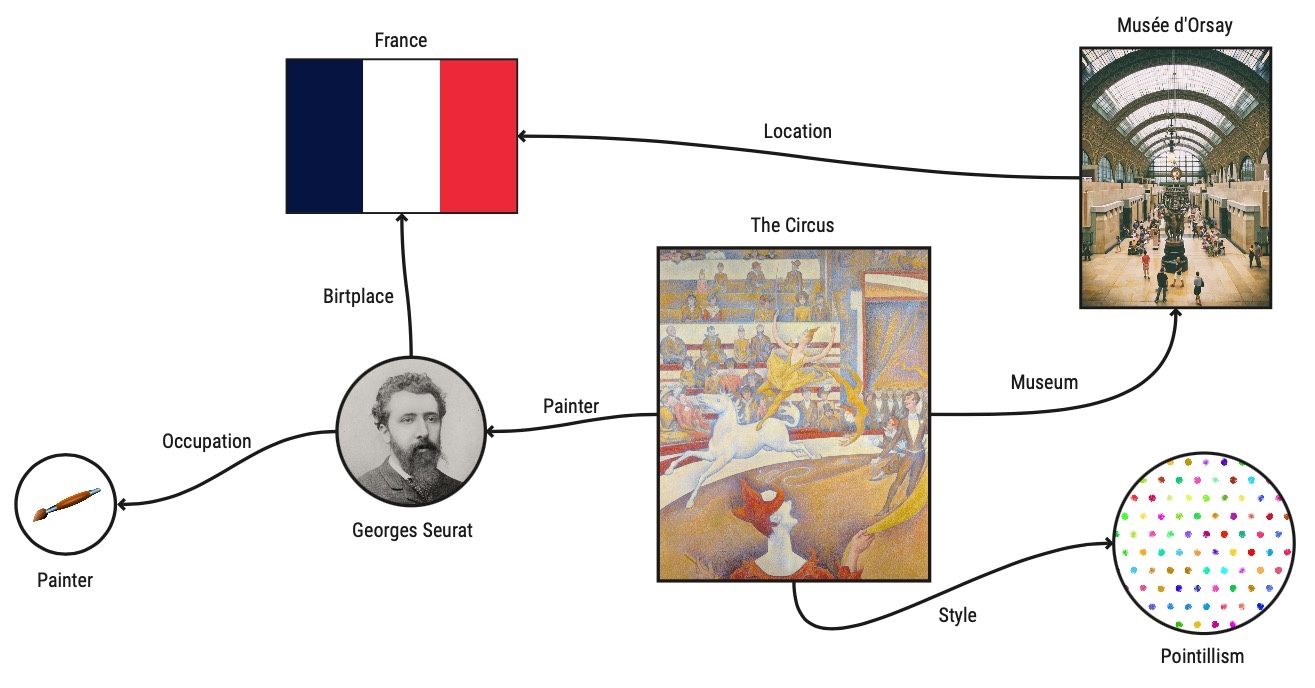
\includegraphics[width=\textwidth]{images/linked_data.jpg}
    \captionsetup{justification=centering}
	\caption{Representation of a web of documents composed according to the spirit of Linked Data}
	\label{fig:linked_data}
\end{figure}

Although several technologies exist to achieve the goals of Linked Data, the use of URIs is essential. After all, since URIs are unique, they can unambiguously reference a particular entity. Practically speaking, the URIs that appear in a Linked Data document can be dereferenced using the HTTP protocol in order to retrieve the underlying entities. For instance, \mintinline{text}{https://stad.gent/id/concept/530010539}, is a URI that can be dereferenced using the HTTP(S) protocol. By dereferencing URI after URI in this way, little by little a - what could be called - \textit{field of information} unfolds, whose semantics can be unambiguously determined by both man and machine. \citep{bizer2011linked}

To clarify the concept of Linked Data, \citet{berners2006linked} put forth four principles to be taken into consideration.
\begin{enumerate}

    \item \textbf{Use URIs as names for things}\\
    The principle of using URIs has already been discussed above.
    
    \item \textbf{Use HTTP URIs so that people can look up those names}\\
    The principle of using the HTTP protocol to dereference URIs was also touched on above. Nevertheless, it is important to reiterate its importance, as there are other protocols besides HTTP for dereferencing URIs. However, these will technically differ from the HTTP protocol, each in its own different ways. For example, not using the ubiquitous Domain Name System (DNS), is, among others, a common practice among alternative protocols. However, in light of clarity and uniformity, as well as for other technical reasons, the HTTP protocol should be adhered to. \citep{berners2006linked}
    
    \item \textbf{When someone looks up a URI, provide useful information, using the standards (RDF, SPARQL)}\\
    Obviously, it would not fit within the spirit of Linked Data to obtain a raw data dump when dereferencing a URI that was included from another document as a \textit{Linked Data link}. The obtained data itself must comply with Linked Data principles. Therefore, there are some standards that clearly indicate how ontologies can be described. Consequently, to enable the construction of applications that deal with Linked Data, it goes without saying that a Linked Data document should be built according to the principles of an existing standard. RDF, RDFS and OWL are common such standards and are therefore discussed further in Sections~\ref{subsec:rdf} and~\ref{subsec:rdfs_owl}. In addition, Section~\ref{subsec:sparql} introduces the SPARQL query interface. After all, large datasets are expected to also provide such interface. \citep{berners2006linked}
    
    \item \textbf{Include links to other URIs so that they can discover more things}\\
    The fourth and final principle, too, is rather obvious. After all, by definition, one can only speak of Linked Data when a document refers to at least one other document. In addition, to help advance the cause of transforming the World Wide Web in its current form into a semantic World Wide Web, aided by the concepts of Linked Data, it is preferable to also include links to documents belonging to other sites. \citep{berners2006linked}
    
\end{enumerate}

In conclusion, Linked Data plays a crucial role in giving meaning to the Web by enabling the interconnection and integration of diverse data sources. By adhering to the principles of unique URIs, dereferencing, linking, and using standardized formats, Linked Data fosters a more structured and interconnected web of knowledge. Examples such as DBpedia\footnote{\href{https://www.dbpedia.org}{https://www.dbpedia.org}}, which provides a structured representation of Wikipedia data, and Friend of a Friend (FOAF), which allows for the description of people and their relationships, illustrate how publishing data as Linked Data benefits from enhanced data discoverability, interlinking with other datasets, and enabling novel applications and insights. Local initiatives like Collections of Ghent (CoGhent\footnote{\href{https://www.collections.gent}{https://www.collections.gent}}), which digitizes art collections from cultural houses in Ghent and will be further discussed in Section~\ref{sec:coghent}, similarly demonstrate the potential of Linked Data for local organizations in contributing to the broader web of knowledge. \citep{auer2007dbpedia} \citep{golbeck2008linking} \citep{van2022publishing}

\subsection{Resource Description Framework}
\label{subsec:rdf}

The idea behind Linked Data is interesting in itself, but does not yet describe exactly how to get started with it. Therefore, this section introduces the Recourse Description Framework (RDF). Developed under the auspices of the World Wide Web Consortium (W3C), RDF is an infrastructure that allows for the construction of Linked Data datasets and their metadata. Consequently, this not only allows data publishers to lay out their data as Linked Data, but also gives data consumers clear guidance on how the data can be understood. Note here that data consumers can be both individuals and computer applications. \citep{miller1998introduction}

An interesting way to understand RDF is to first make a jump to the English language. Take the sentence below:
\begin{center}
    \textbf{The birthplace of Georges Seurat is France.}
\end{center}
According to English grammar, the \textit{who} or \textit{what} around which a sentence revolves, is called the subject of the sentence. Therefore, when looking at the sentence above, \textit{Georges Seurat} is its subject. In addition, the part of a sentence that gives more information about the subject, is referred to as the predicate, making \textit{the birthplace} the predicate in the above sentence. Finally, the matching value complementing the predicate and completing the sentence, is also of importance. Logically, in the case of the sentence above, that would be \textit{France}. Together, these three components form the most basic building blocks of a sentence. In fact, no matter their lengths, combined, they will always establish a piece of knowledge, exactly what RDF also seeks to accomplish. \citep{powers2003practical}

The building blocks of RDF data are basically exactly the same as those of linguistic sentences. After all, they are also three in number and even partly share the same names. Moreover, much like with sentences, combined, they form a single yet very clear piece of knowledge. Unlike the English language, however, they are not referred to as sentences. Rather, they are called triples. \citep{powers2003practical}
\begin{itemize}

    \item \textbf{Resource}\\
    \cite{miller1998introduction} defines a resource as any object that is uniquely identifiable by a URI. This enables it to come in different forms: as a web page, as an entire website or simply as any resource on the Web that conveys information in one way or another. \citep{candan2001resource}
    
    To make the comparison with the English language again, in a triple, the resource corresponds to the subject in a sentence. Moreover, in practice, the term \textit{subject} is often preferred over \textit{resource}. \citep{powers2003practical}

    \item \textbf{Property Type}\\
    A property type, or simply a property, introduces a specific aspect, characteristic, attribute, or relationship of a resource. A property type always expects a value to ultimately define the piece of knowledge represented by a triple. \citep{candan2001resource} \citep{miller1998introduction}
    
    As for property types, in practice, the corresponding term from the English language, \textit{predicate}, is also frequently used as opposed to the more theoretical \textit{property type}. \citep{powers2003practical}

    \item \textbf{Value}\\
    A value resolves the concept or relationship initiated by a property type. In this way, it captures the knowledge conveyed by the triple. Values can be represented as text strings, numbers, or any atomic data. However, they can also be resources themselves. This characteristic allows triples therefore to be the building blocks of a web of knowledge. \citep{miller1998introduction}
    
    It is evident that a value in a triple corresponds to a value in an English sentence. However, in practice, the term \textit{object} is often preferred. \citep{powers2003practical}
    
\end{itemize}

While triples convey a clear and distinct piece of knowledge, a collection of triples can naturally convey a more comprehensive knowledge. Such a collection of triples, interconnected by values that are themselves resources, is also referred to as an \textit{RDF description}. Figure~\ref{fig:rdf_description} illustrates what such an RDF description might look like. Additionally, it is important to note that each of its components, whether it be a resource, property type, or value, does not necessarily have to be a digital concept. After all, Web assets can perfectly represent real-life concepts. \citep{miller1998introduction} \citep{candan2001resource}

\begin{figure}[htbp]
    \centering
	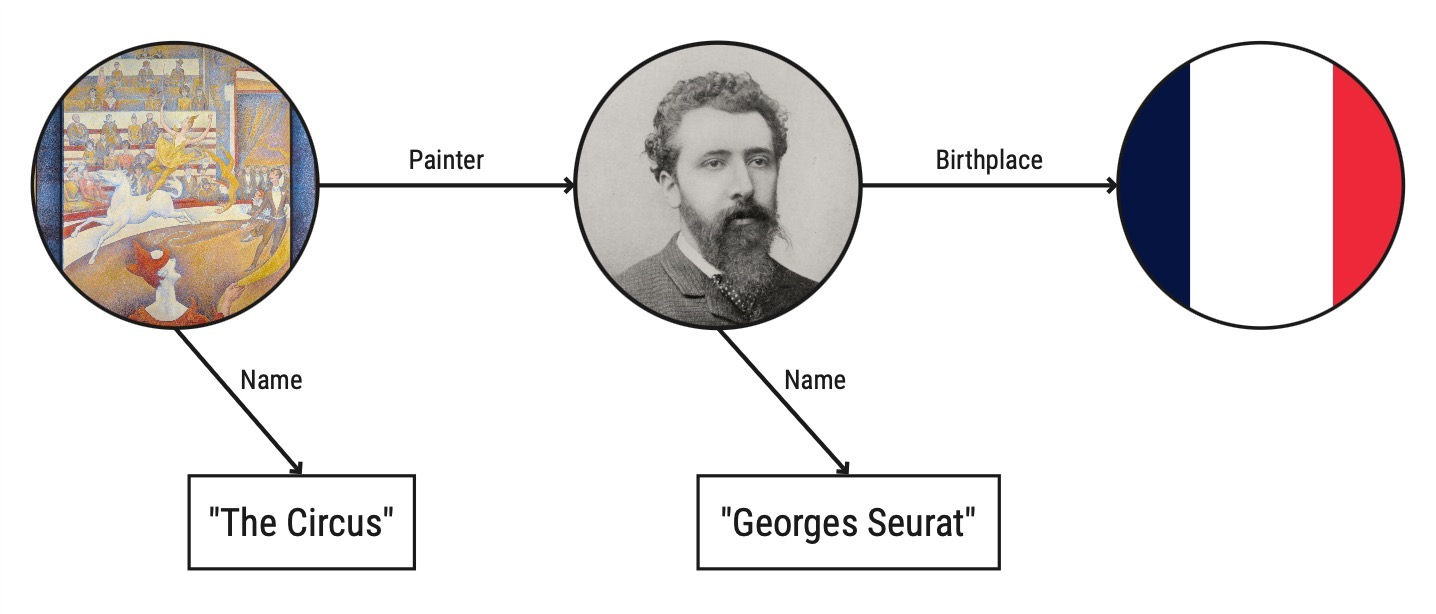
\includegraphics[width=\textwidth]{images/rdf_description.jpg}
    \captionsetup{justification=centering}
	\caption{Representation of an RDF description}
    \caption*{Circles represent resources, arrows represent property types and values are situated at the end of arrows}
	\label{fig:rdf_description}
\end{figure}

Clearly, different terms exist to denote the same RDF concepts. For instance, in addition to the synonyms mentioned above, in literature, the term \textit{statement} is sometimes preferred over \textit{triple}. However, in light of uniformity and clarity, throughout the rest of this text, the terms \textit{triple}, \textit{subject}, \textit{predicate} and \textit{object} will be used instead of their counterparts. \citep{candan2001resource}

\subsection{Resource Description Framework Syntax}
\label{subsec:rdf_syntax}

What constitutes RDF exactly, should be clear by now, but the question of how to actually write down RDF descriptions, still remains to be answered. Therefore, this section introduces some RDF syntaxes. However, since they are not the focus of this research, they will not be discussed in detail. Instead, their outlines will be illustrated by presenting the RDF description from Figure~\ref{fig:rdf_description} in the syntax in question. Incidentally, since the schema presented in Figure~\ref{fig:rdf_description} also has clear guidelines on how to be used, in itself, it also qualifies as an RDF syntax, albeit a graphical one. \citep{miller1998introduction}

All the syntaxes to be discussed are instantiations of the RDF Model and Syntax Specification, providing concrete implementations. However, the first syntax stands apart from the rest as it primarily serves as a notation recommendation for humans to express RDF descriptions in a manner that is unambiguous yet simple. Unlike the other syntaxes, this particular one is not intended for machine consumption. Code Fragment~\ref{lst:human_rdf_syntax} demonstrates how the RDF descriptor, as schematically depicted in Figure~\ref{fig:rdf_description}, can be represented using this human-centric syntax. In this representation, resources are enclosed in straight brackets, while property types are represented by arrows. Furthermore, the representation of values varies depending on their types. As denoted, resources are encapsulated within brackets. However, if the values are atomic in nature, they are simply enclosed in quotation marks. \citep{miller1998introduction}

\begin{listing}[htbp]
    \begin{minted}[samepage]{text}
[The Circus] ------name--------> "The Circus"
[The Circus] ------painter-----> [Georges Seurat]
[Georges Seurat] --name--------> "Georges Seurat"
[Georges Seurat] --birthplace--> [France]
    \end{minted}
    \caption{RDF description depicted using a human-centric RDF syntax}
    \label{lst:human_rdf_syntax}
\end{listing}

The example from Code Fragment~\ref{lst:human_rdf_syntax} is easy to read, but at the same time rather confusing. Indeed, certain resource names correspond to certain atomic values. One could of course try to give the resources a more generic name to indicate what exactly the resource in question means. However, that would make little sense given the way the following machine-readable RDF syntaxes refer to resources. After all, they use URIs, allowing for a more clear distinction between resources and atomic values.

\begin{itemize}

    \item \textbf{N-Triples}\\
    TODO (see Code Fragment~\ref{lst:n_triples_syntax}

    \begin{listing}[htbp]
        \begin{minted}[samepage, fontsize=\footnotesize]{turtle}
<http://example.org/The_Circus> <http://example.org/name> "The Circus" .
<http://example.org/The_Circus> <http://example.org/painter> <http://example.org/Georges_Seurat> .
<http://example.org/Georges_Seurat> <http://example.org/name> "Georges Seurat" .
<http://example.org/Georges_Seurat> <http://example.org/birthplace> <http://dbpedia.org/resource/France> .
        \end{minted}
        \caption{RDF description depicted using the N-Triples syntax}
        \label{lst:n_triples_syntax}
    \end{listing}

    \item \textbf{N3}\\
    TODO (see Code Fragment~\ref{lst:n3_turtle_syntax}

    \begin{listing}[htbp]
        \begin{minted}[samepage]{turtle}
@prefix ex: <http://example.org/> .
@prefix dbp: <http://dbpedia.org/resource/> .

ex:The_Circus ex:name "The Circus" .
ex:The_Circus ex:painter ex:Georges_Seurat .
ex:Georges_Seurat ex:name "Georges Seurat" .
ex:Georges_Seurat ex:birthplace dbp:France .
        \end{minted}
        \caption{RDF description depicted using the N3 and Turtle syntaxes}
        \label{lst:n3_turtle_syntax}
    \end{listing}

    \item \textbf{Turtle}\\
    TODO (see Code Fragment~\ref{lst:n3_turtle_syntax}

    \item  \textbf{XML/RDF}\\
    TODO (see Code Fragment~\ref{lst:xml_syntax})

    \begin{listing}[htbp]
        \begin{minted}[samepage]{xml}
<rdf:RDF xmlns:rdf="http://www.w3.org/1999/02/22-rdf-syntax-ns#"
         xmlns:ex="http://example.org/"
         xmlns:dbp="http://dbpedia.org/resource/">
  <rdf:Description rdf:about="http://example.org/The_Circus">
    <ex:name>The Circus</ex:name>
    <ex:painter rdf:resource="http://example.org/Georges_Seurat"/>
  </rdf:Description>
  <rdf:Description rdf:about="http://example.org/Georges_Seurat">
    <ex:name>Georges Seurat</ex:name>
    <ex:birthplace rdf:resource="http://dbpedia.org/resource/France"/>
  </rdf:Description>
</rdf:RDF>
        \end{minted}
        \caption{RDF description depicted using the XML/RDF syntax}
        \label{lst:xml_syntax}
    \end{listing}

    \item \textbf{JSON-LD}
    TODO (see Code Fragments~\ref{lst:json_ld_nested_syntax},~\ref{lst:json_ld_spread_syntax} and~\ref{lst:json_ld_graph_syntax}

        \begin{listing}[htbp]
        \begin{minted}[samepage]{jsonld}
{
  "@context": {
    "ex": "http://example.org/",
    "dbp": "http://dbpedia.org/resource/"
  },
  "@id": "ex:The_Circus",
  "ex:name": "The Circus",
  "ex:painter": {
    "@id": "ex:Georges_Seurat",
    "ex:name": "Georges Seurat",
    "ex:birthplace": "dbp:France"
  }
}
        \end{minted}
        \caption{RDF description with nested objects depicted using the JSON-LD syntax}
        \label{lst:json_ld_nested_syntax}
    \end{listing}

        \begin{listing}[htbp]
        \begin{minted}[samepage, escapeinside=||]{jsonld}
|Document 1:|
{
  "@context": {
    "ex": "http://example.org/"
  },
  "@id": "ex:The_Circus",
  "ex:name": "The Circus",
  "ex:painter": "ex:Georges_Seurat"
}

|Document 2:|
{
  "@context": {
    "ex": "http://example.org/",
    "dbp": "http://dbpedia.org/resource/"
  },
  "@id": "ex:Georges_Seurat",
  "ex:name": "Georges Seurat",
  "ex:birthplace": "dbp:France"
}
        \end{minted}
        \caption{RDF description spread over two documents depicted using the JSON-LD syntax}
        \label{lst:json_ld_spread_syntax}
    \end{listing}

            \begin{listing}[htbp]
        \begin{minted}[samepage]{jsonld}
{
  "@context": {
    "ex": "http://example.org/",
    "dbp": "http://dbpedia.org/resource/"
  },
  "@graph": [
    {
      "@id": "ex:The_Circus",
      "ex:name": "The Circus",
      "ex:painter": {
        "@id": "ex:Georges_Seurat"
      }
    },
    {
      "@id": "ex:Georges_Seurat",
      "ex:name": "Georges Seurat",
      "ex:birthplace": {
        "@id": "dbp:France"
      }
    }
  ]
}
        \end{minted}
        \caption{RDF description as a graph depicted using the JSON-LD syntax}
        \label{lst:json_ld_graph_syntax}
    \end{listing}
    
\end{itemize}

\subsection{Resource Description Framework Schema and Web Ontology Language}
\label{subsec:rdfs_owl}

TODO

\subsection{SPARQL and Query Interfaces}
\label{subsec:sparql}

TODO

\subsection{Challenges and Advantages}
\label{subsec:challenges_advantages}

TODO

\section{Link-Traversal-based Query Processing}

TODO

\section{Comunica}

TODO

\section{Collections of Ghent}
\label{sec:coghent}

TODO
\chapter*{Conclusion}
\chaptermark{Conclusion}
\addcontentsline{toc}{chapter}{Conclusion}  

TODO

\phantomsection
\section*{Ethical and social reflection}
\addcontentsline{toc}{section}{Ethical and social reflection}  

This section is required only for industrial engineering courses. The location of this section slightly differs from the order prescribed by the faculty. We recommend making this reflection as part of the conclusion because it allows you to easily reference results in your master's thesis itself.

You can look up more information at https://www.sdgs.be/nl/sdgs

\renewcommand\bibname{References}
\bibliography{references}


\pagestyle{numberless} 
\pagestyle{empty}
\begin{appendices}
\section*{Appendix A}
\addcontentsline{toc}{section}{Appendix A}  

TODO

\newpage
\section*{Appendix B}
\addcontentsline{toc}{section}{Appendix B}  

TODO

\end{appendices}


\end{document}
